%-----------------------------------------------------------------------------
%
%               Template for sigplanconf LaTeX Class
%
% Name:         sigplanconf-template.tex
%
% Purpose:      A template for sigplanconf.cls, which is a LaTeX 2e class
%               file for SIGPLAN conference proceedings.
%
% Guide:        Refer to "Author's Guide to the ACM SIGPLAN Class,"
%               sigplanconf-guide.pdf
%
% Author:       Paul C. Anagnostopoulos
%               Windfall Software
%               978 371-2316
%               paul@windfall.com
%
% Created:      15 February 2005
%
%-----------------------------------------------------------------------------


%\documentclass[preprint]{sigplanconf}
\documentclass[10pt]{sigplanconf}

% The following \documentclass options may be useful:
%
% 10pt          To set in 10-point type instead of 9-point.
% 11pt          To set in 11-point type instead of 9-point.
% authoryear    To obtain author/year citation style instead of numeric.

\usepackage{yfonts}
\usepackage{amsmath}
\usepackage{amsthm}
\usepackage{amssymb}
%\usepackage{mathpartir}
\usepackage[colorlinks=true,
citecolor=citec,
linkcolor=linkc,
urlcolor=urlc,
]{hyperref}
\usepackage{url}
\usepackage{graphics}
\usepackage{graphicx}
\usepackage{wasysym}
\usepackage{harmony}
\usepackage{marvosym}
\usepackage{multirow}
\usepackage{xspace}
\usepackage[nameinlink,nosort]{cleveref}
\usepackage{xeCJK}
\usepackage[usenames,dvipsnames]{xcolor}
\usepackage[utopia]{mathdesign}
\usepackage{natbib}
\usepackage{ulem}
\usepackage[mathcal]{euscript}
\usepackage[linesnumbered,ruled]{algorithm2e}

\renewcommand{\UrlBreaks}{\do\/\do\a\do\b\do\c\do\d\do\e\do\f\do\g\do\h\do\i\do\j\do\k\do\l\do\m\do\n\do\o\do\p\do\q\do\r\do\s\do\t\do\u\do\v\do\w\do\x\do\y\do\z}


% ____________________________________________________________
% Listings Package Configuration
% \usepackage[scaled]{beramono}

%\renewcommand*\ttdefault{txtt}
\usepackage[T1]{fontenc}

\definecolor{citec}{RGB}{128,0,64}
\definecolor{linkc}{RGB}{0,64,128}
\definecolor{urlc} {RGB}{128,64,0}

\setCJKmainfont{HeiseiMinStd-W5}[Path = ./]
\setmonofont{Inconsolata-Regular}[Path = ./]
% This Deep Tex Voodoo is from
%   <http://www.latex-community.org/forum/viewtopic.php?f=5&t=2072>
% It's purpose is to make \lstinline normal size, without affecting
% \lstinputlisting.  It seems to work but I have no idea how or why,
% and I rather hope never to learn.
%\makeatletter
%\lst@AddToHook{TextStyle}{\let\lst@basicstyle\ttfamily\normalsize}
%\makeatother

\begin{document}

\conferenceinfo{SIGBOVIK '19}{Pittsburgh, PA, USA}
\copyrightyear{2019}
\copyrightdata{}

\titlebanner{banner above paper title}        % These are ignored unless
\preprintfooter{short description of paper}   % 'preprint' option specified.

\title{
Which ITG Stepcharts are Bracket-Jumpiest?: \\
In Which They Milk the \\
「A Boring Follow-Up Paper to \\
``Which ITG Stepcharts are Turniest?'' \\
Titled, ``Which ITG Stepcharts are Crossoveriest and/or Footswitchiest?''」\\
Series for All Its Worth in Publication Count After All \\
%That `Boring' Stuff Was Part of the Title, BTW. \\
%So was that. And that, and this too. \\
%You got it all, right? \\
%Or Just, ``More Boring Crap about ITG'', for Short. \\
%Oh, That Was Also Part of the Title.
}
% \subtitle{\em The Randomly-Scoped Lambda Calculus}
% \subtitle{Subtitle Text, if any}

\authorinfo{Ben Blum}{}{bblum@alumni.cmu.edu}

\maketitle

\begin{abstract}
	%ITG is a popular dance game in which players step on arrows while listening to music. The arrow patterns, indicated by a {\em stepchart}, may range among any level of complexity and difficulty. Among the many factors contributing to a stepchart's difficulty is how much the player must turn from side to side.
	%Other more obvious factors, such as raw speed, have been well studied in prior work.
	%This paper presents an analytic study of this {\em turniness} factor.
	%We study the turniness of many existing stepcharts, and present a novel (but unsurprising) approach to automatically generating maximally (or minimally) turny charts.
	%Among real-world songs, we find stepcharts with overall turniness ranging from 0\% to 81.33\% of the theoretical maximum.

In which I break last last year's promise of no future work.

\end{abstract}

\category{D.D.R.}{Exercise and Fitness}{Arcade Dance Games}

\keywords
bracket, groove, in, jumps, the


\section{Introduction}

Recent work by \cite{dril}
%[W. Dril et al., 2019]
proposed the hypothesis that
recent stepchart authors have grown bored with the array of technical ITG step patterns
documented to date \cite{turniness,crossoveriness},
and have moved on to break the old model's one-foot-per-arrow assumption to allow for even more technical patterns yet.
I paraphrase their main conclusion as follows:

\begin{center}
	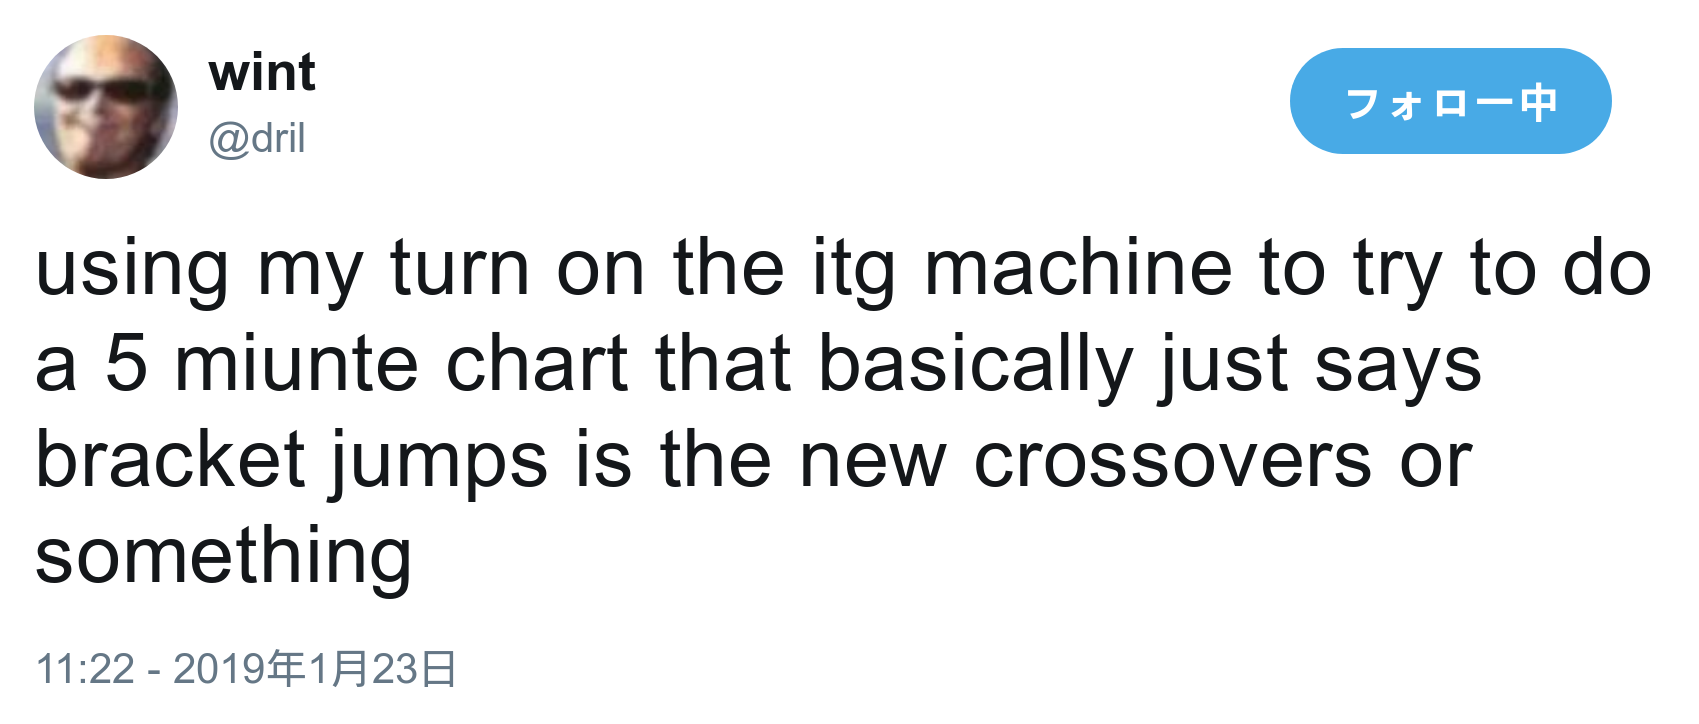
\includegraphics[width=0.42\textwidth]{using-my-turn.png}
\end{center}

All good researchers know that when rise the standards for software or hardware performance
(or stepchart trickiness, as the case may be),
they must revisit their own work to prove its ongoing relevance to the research (dance) community at large.
Thus I must regrettably break the promise \sout{I} the authors set forth in \cite{crossoveriness}
(see \Cref{fig:you-stutid-fuckass})
and revisit \sout{my} their old future work section
(XXX: they said to change any first-person ``our prior work''
stuff like this for double-blind review but like cmon this makes no sense?
theyll totally see through this
(TODO: maybe email the PC chair for advice?
(FIXME: make sure to remove these comments before the camera-ready deadline!!))),
extending it to handle these new so-called ``bracket'' jumps.

\begin{figure}[t]
	\hspace{-2em}\includegraphics[angle=270,width=0.54\textwidth]{../2/paper.pdf}
	\caption{(yeah i reused this joke from last time ok deal)}
	\label{fig:you-stutid-fuckass}
\end{figure}

%%%%%%%%%%%%%%%%%%%%%%%%%%%%%%%%%%%%%%%%%%%%%%%%%%%%%%%%%%%%%%%%%%%%%%%%%%%%%%%%

\section{Overview}

% TODO: go through this paper and make every *other* instance of "bracket-jump" hyphenated

What, then, is a bracket jump (which I shall \textit{not}, henceforth, abbreviate for brevity)?
Put simply, whenever two arrow-shaped obstacles proceed simultaneously towards the protagonist directional indicator targets
(see \cite{turniness}),
while a novice player might think they must step with both feet at once, one for each arrow,
experts often find it more convenient (i.e., less overall foot motion) to use whichever single foot is closer at the time
to hit both arrows by
triggering one arrow's sensor with the heel and the other with the little bitty toesies.
Pads are typically constructed with a small triangular metal bracket at the corner of each arrow panel,
as shown in \Cref{fig:bracker-detail},
which the bridge of the foot must cross to achieve this, hence the name ``bracket jump''.
In case my prose explanation is not up to snuff, I also show in \Cref{fig:how-2-bracket}
a high-quality graphics render of a player's typical foot positions during a down+right bracket jump (henceforth ``DR'', et cetera).

The reader, or stepper,
may notice the extreme angle of footing depicted in the latter figure,
which is necessary to reliably trigger both pad sensors.
Accordingly, this maneuver is comfortable (and hence preferable to a normal jump)
only if the player is already facing in roughly the same direction \cite{turniness}.
%after stepping any preceding patterns.
The next section will attempt to codify (ahem) when
preceding patterns encourage the player to bracket rather than jump,
and thereby identify how ``bracket jumpy'' each chart is.

\begin{figure}[t]
	\begin{center}
		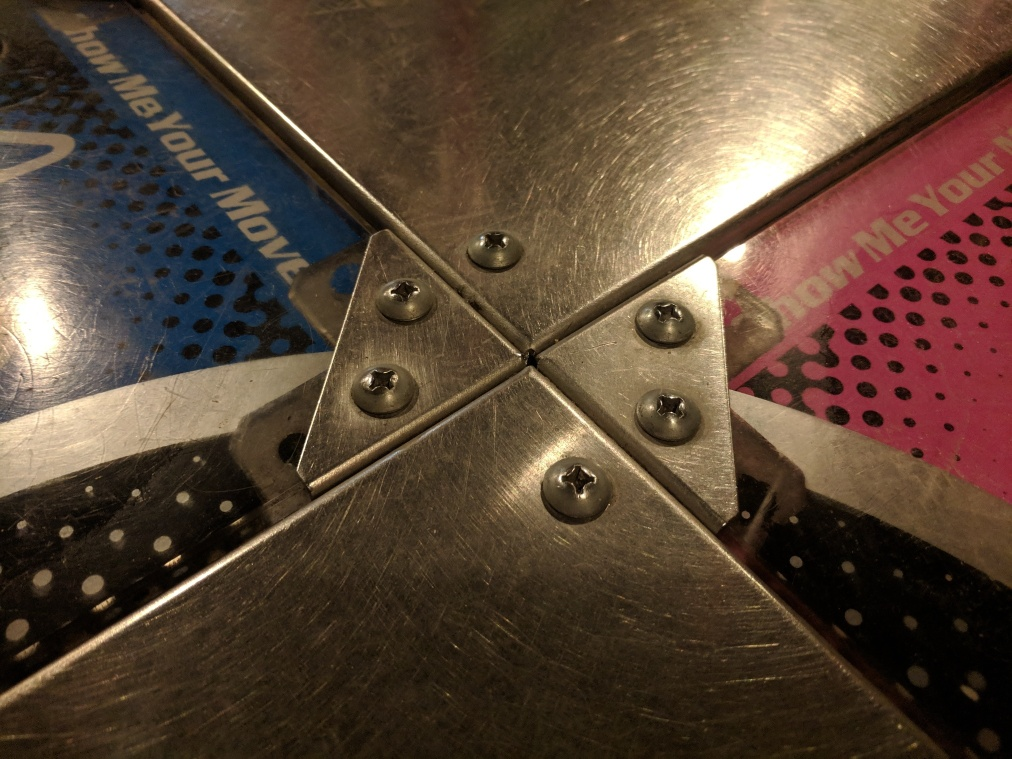
\includegraphics[width=0.48\textwidth]{jims-pix.jpg}
	\end{center}
	\caption{Detail of metal corner brackets, this paper's namesake. Photo credit {\tt JIM}.}
	\label{fig:bracker-detail}
\end{figure}

\begin{figure}[h]
	\begin{center}
		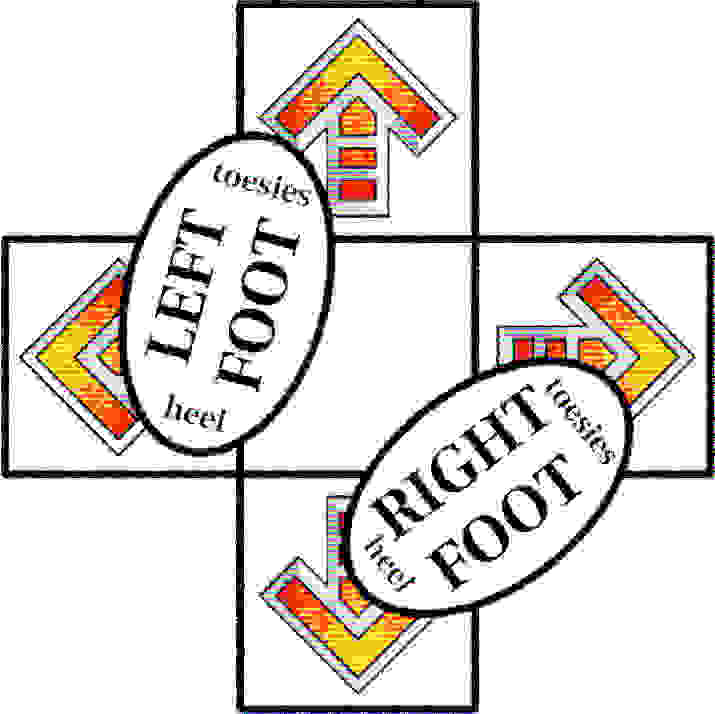
\includegraphics[width=0.48\textwidth]{how-2-bracket.jpg}
	\end{center}
	\caption{Down+right bracket jump real-world example.}
	\label{fig:how-2-bracket}
\end{figure}

%%%%%%%%%%%%%%%%%%%%%%%%%%%%%%%%%%%%%%%%%%%%%%%%%%%%%%%%%%%%%%%%%%%%%%%%%%%%%%%%

\section{Analyzing Bracket-Jumpiness}
\label{sec:analyzing}

I extended the crossoveriness et cetera algorithm from \cite{crossoveriness} to reason about jumps,
which previously it treated all identically,
ignoring the arrows involved and allowing the player to reset her footing as desired.
Now, it considers LD, LU, DR, and UR jumps as potentially bracketable,
allowing the player to continue a stream of alternating feet uninterrupted through.

\textit{Confession.}
When I was first brainstorming this project,
I had some grand visions of unifying the turniness algorithm \cite{turniness}---which
accounts for U/D steps to figure out how far the player must turn each step,
but has no idea which way the player is actually facing at any given time---with
the crossoveriness one
(cited just above; cmon how much do you want me to repeat these, gimme a break)---which
totally ignores U/D steps and just figures out which arrows the left and right feet must each step---in
some theoretically beautiful way to produce the unquestionably perfect footing sequence for each jump.
%
However, as I was considering how to incorporate features from last time's algorithm,
potentially allowing crossover brackets (\Cref{sec:xover-brackers})
and footswitch brackets (\Cref{sec:fs-brackers}),
I realized that ultimately there would be no restrictions on what jumps were bracketable;
the algorithm would oops simply twist and turn as much as necessary to bracket everything,
and this paper would become ``Which ITG Stepcharts Have the Most Jumps?'', and like who wants to read that.

One may think to simply try either bracketing each jump or not
and seeing what combination gives the minimum turniness result,
but since whether to bracket each jump or not affects subsequent steps' footing,
each choice cannot in general be solved independently,
and I hope you can see where this is going.
Now the last time I tried to solve an exponentially-sized problem, it took me 7 years
(and I still ended up with a pile of heuristics after all anyway)
\cite{landslide-thesis},
so considering I started this project a week before the deadline,
I instead to just code up a bunch of ad-hoc rules to handle all the different bracket jump patterns
that occurred to me to write test cases for.

As before, the code is available at \url{https://github.com/bblum/sigbovik/blob/master/itg/code/ITG.hs}.
To give an idea of how much its elegance has been despoiled % hi william
since the last version:
98 lines of Haskell (which computed crossovers, footswitches, jacks, doubleswitches, \textit{and} crossover footswitches)
has grown to 248 lines (just to handle this one. new. feature),
and the once-simple datatype definition of

\newcommand\hilight[2]{\color{#1}#2\color{black}\xspace}
\definecolor{pink}{RGB}{128,0,192}
\definecolor{orange}{RGB}{192,96,0}
\definecolor{olivegreen}{RGB}{0,127,32}
\definecolor{brickred}{RGB}{192,0,0}
\definecolor{commentblue}{RGB}{0,128,192}

\begin{center}
	\texttt{\hilight{orange}{data}~\hilight{olivegreen}{Step} =
	\hilight{brickred}{L} |
	\hilight{brickred}{D} |
	\hilight{brickred}{U} |
	\hilight{brickred}{R} |
	\hilight{brickred}{Jump}}
\end{center}

has become:


\begin{center}
	\begin{tabular}{l}
	\texttt{\hilight{orange}{data}~\hilight{olivegreen}{Arrow} =
	\hilight{brickred}{L} |
	\hilight{brickred}{D} |
	\hilight{brickred}{U} |
	\hilight{brickred}{R}} \\
	\texttt{\hilight{orange}{data}~\hilight{olivegreen}{Jump} =
	\hilight{brickred}{LD} |
	\hilight{brickred}{LU} |
	\hilight{brickred}{DR} |
	\hilight{brickred}{UR} |
	\hilight{brickred}{LR} |
	\hilight{brickred}{DU} |
	\hilight{brickred}{Other}} \\
	\texttt{\hilight{orange}{data}~\hilight{olivegreen}{Step} =
	\hilight{brickred}{A} \hilight{olivegreen}{Arrow} |
	\hilight{brickred}{J} \hilight{olivegreen}{Jump}} \\
	\texttt{\hilight{orange}{data}~\hilight{olivegreen}{Foot} =
	\hilight{brickred}{LeftFoot} |
	\hilight{brickred}{RightFoot}} \\
	\end{tabular}
\end{center}

In lieu of an algorithm listing, I'll simply show some of those most notable test cases in pictures and explain in prose how I handle them.


\subsection{Basic Examples}

Figure \Cref{fig:bracket-example}(a) shows a simple example where every jump (blue)
can be bracketed by the right foot,
alternating with 

%%%%%%%%%%%%%%%%%%%%%%%%%%%%%%%%%%%%%%%%%%%%%%%%%%%%%%%%%%%%%%%%%%%%%%%%%%%%%%%%

\section{Evaluation}


%%%%%%%%%%%%%%%%%%%%%%%%%%%%%%%%%%%%%%%%%%%%%%%%%%%%%%%%%%%%%%%%%%%%%%%%%%%%%%%%

\section{Discussion}

% TODO tings to talk about

% authors seem to know it's easy to overdo -- see, "Stupid" and "I'm sorry" as chart authors in some of the top charts

% many old charts written without regard to jump patterning can be bracker anyway, see OWA (which just makes the list bc it's long)
% - have a figure of OWA in the strema that shows the *non* bracketable stream jumps
% - make a test case that captures these and shows indeed they are not brackets

% temporal analysis of pack age vs bracker density

% other charts of note
% - chicago timing / electrical paradise: bracketiest chart where *ALL* jumps are brackets (BJJ%=100) -- quite tasteful actually!
% - encore is 2nd place lmao

% conclusion: BJJ% is sa better measure of chart funness than BJS%?

\section{Never Work}

The only thing that impresses the research community more than overdelivering on your future work promises
is to overdeliver twice; hence, I shamelessly reuse the joke of this section name from last time.

\subsection{Crossover Brackets}
\label{sec:xover-brackers}

\subsection{Footswitch Brackets}
\label{sec:fs-brackers}

I put this section here only just so I could have something to forward-reference back in \Cref{sec:analyzing}.
I always wanted to do that, you know?
I mean, footswitch brackets are also a real thing, but still. $\bar{~~}$\textbackslash\_(ツ)\_/$\bar{~~}$
% not-to-to: put a pict anyway? if you find one
% actually, joke comes off better w/o

\subsection{UI}

It would be cool to integrate this (and the preceding two algorithms \cite{turniness,crossoveriness})
into
%Simply Love \cite{simplylove}, or whatever
the community's prevailing stepmania theme.
%may be in the future.
Currently, as shown in \Cref{fig:songpreview}(a),
the song preview screen wastes considerable space displaying the count of irrelevant chart aspects
such as mines (now used primarily for signaling the presence of footswitches)
and hands (now mostly stepped with the feet by bracketing anyways).
I bet the community might actually pay attention to my work---the holy grail of research, honestly---if
popular themes used it to show precisely how technical a chart was, as in (b).

\begin{figure}[t]
	\begin{tabular}{c}
	
\includegraphics[width=0.46\textwidth]{song-info.png} \\
		(a) Current state-of-the-art.
		\\
		\\
	
\includegraphics[width=0.46\textwidth]{song-info-better.png} \\
		(b) Artist's conception.
	\end{tabular}
	\caption{Song info preview panel for a recent bracket jump-heavy stepchart \cite{divine}.}
	\label{fig:songpreview}
\end{figure}

\subsection{Obligatory Machine Learning Section}

I guess you could skip all this fiddly ``algorithm'' stuff by
hopping on the pads yourself for a few rounds, playing a variety of technical charts,
and just training a neural network based on how you stepped the patterns.
It would probably even learn to fake crossovers more at the ends of songs than at the beginnings,
where you're more likely to be physically tired.
But like, do you really want that kind of bias in your dataset?

Remember kids, friends don't let friends use ML for problems that are more fun to solve by hand.

\section{Conclusion}

I never know what to put down here. Much love to the community..!


%%%%%%%%%%%%%%%%%%%%%%%%%%%%%%%%%%%%%%%%%%%%%%%%%%%%%%%%%%%%%%%%%%%%%%%%%%%%%%%%

\bibliographystyle{abbrvnat}
\bibliography{citations}

\end{document}
